\documentclass[oneside,fleqn,11pt]{book}
\usepackage[a4paper, total={7.2in, 10.3in}]{geometry}
\usepackage{tikz}
\usetikzlibrary{calc}
\usepackage{setspace}
\usepackage{graphicx}
\usepackage{amsmath}
\usepackage{amssymb}
\DeclareMathOperator\dx{\mathrm{d}\mathit{x}}
\DeclareMathOperator\dy{\mathrm{d}\mathit{y}}
\DeclareMathOperator\dt{\mathrm{d}\mathit{t}}
\DeclareMathOperator\dv{\mathrm{d}\mathit{v}}
\DeclareMathOperator\dtheta{\mathrm{d}\mathit{\theta}}
\DeclareMathOperator\cis{cis}
\DeclareMathOperator\sech{sech}
\DeclareMathOperator\csch{csch}
\DeclareMathOperator\arsinh{arsinh}
\DeclareMathOperator\arcosh{arcosh}
\DeclareMathOperator\artanh{artanh}
\DeclareMathOperator\Nset{\mathbb{N}}
\DeclareMathOperator\Zset{\mathbb{Z}}
\DeclareMathOperator\Qset{\mathbb{Q}}
\DeclareMathOperator\Rset{\mathbb{R}}
\DeclareMathOperator\Iset{\mathbb{I}}

\usepackage{pgfplots}
\graphicspath{ {./images/} }
\usepackage{bookmark}
\setcounter{tocdepth}{0}
\usepackage{import}
\usepackage{mathtools}
\usepackage{hyperref}
\usepackage{blindtext}

\counterwithin*{chapter}{part}
\newcommand*{\Part}[2][\partheading]{%
  \refstepcounter{part}%
  \def\partheading{#2}%
  \part*{#2}%
  \addcontentsline{toc}{part}{#1}%
}


\DeclarePairedDelimiter{\ceil}{\lceil}{\rceil}
\hypersetup{
	colorlinks   = true, %Colours links instead of ugly boxes
	urlcolor     = blue, %Colour for external hyperlinks
	linkcolor    = black, %Colour of internal links
	citecolor   = red %Colour of citations
}

\newcommand{\tikzAngleOfLine}{\tikz@AngleOfLine}
\def\tikz@AngleOfLine(#1)(#2)#3{%
	\pgfmathanglebetweenpoints{%
		\pgfpointanchor{#1}{center}}{%
		\pgfpointanchor{#2}{center}}
	\pgfmathsetmacro{#3}{\pgfmathresult}%
}

% math font
\usepackage{amsmath}
\usepackage{amssymb}
\usepackage{amsthm}
\usepackage{mathtools}
%\usepackage{arev}

% color
\usepackage[table]{xcolor}

\usepackage[many]{tcolorbox}
\usepackage{pifont}
\usepackage{hyperref}
\hypersetup{%
	linktoc=all,%
	bookmarksnumbered,%
	bookmarksopen,%
	hidelinks}
\usepackage{bookmark}
\bookmarksetup{
	addtohook={%
		\ifnum\bookmarkget{level}=0%
		\bookmarksetup{color=red}%
		\fi%
		\ifnum\bookmarkget{level}=1%
		\bookmarksetup{color=blue}%
		\fi%
		\ifnum\bookmarkget{level}=2%
		\bookmarksetup{color=teal}%
		\fi}}
% enumerate
\usepackage[inline]{enumitem}
\usepackage{multicol}
\usepackage[inline]{enumitem}
\usepackage{tasks}
\usepackage{caption}
\usepackage{subcaption}
\usepackage{cancel}
\usepackage{bm}

\renewcommand\rmdefault{ptm}
\renewcommand\sfdefault{ptm}

\tcbset{
	colframe=magenta,
	colback=magenta!12!white,
	boxed title style={colback=magenta},
	breakable,
	enhanced,
	sharp corners,
	boxsep=1pt,
	attach boxed title to top left={yshift=-\tcboxedtitleheight,  yshifttext=-.75\baselineskip},
	boxed title style={boxsep=1pt,sharp corners},
	fonttitle=\bfseries\sffamily,
	drop lifted shadow
}
\newtcolorbox{solution}[1][]{
	no shadow,
	top=2ex,
	boxrule=0pt,
	leftrule=1.4pt,
	title={Solution},
	colframe=green!79!blue,
	colback=green!12!white,
	boxed title style={colback=green!79!blue},
	overlay unbroken and first={
		\node[below right,font=\small,color=magenta,text width=.8\linewidth]
		at (title.north east) {#1};
	}
}
\newtcolorbox[auto counter,number within=chapter,number format=\arabic]{activity}[1][]{
	title={Activity~\thetcbcounter},
	colframe=green,
	colback=green!22!white,
	coltitle=black,
	boxed title style={colback=green},
	overlay unbroken and first={
		\node[below right,font=\small,color=green,text width=.8\linewidth]
		at (title.north east) {#1};
	}
}
\newtcolorbox[auto counter,number within=chapter,number format=\arabic]{definition}[1][]{
	title={Definition~\thetcbcounter},
	colframe=blue,
	colback=blue!12!white,
	boxed title style={colback=blue},
	overlay unbroken and first={
		\node[below right,font=\small,color=blue,text width=.8\linewidth]
		at (title.north east) {#1};
	}
}
\newtcolorbox[auto counter,number within=chapter,number format=\arabic]{theorem}[1][]{
	title={Theorem~\thetcbcounter},
	colframe=violet,
	colback=violet!12!white,
	fontupper=\itshape,
	boxed title style={colback=violet},
	overlay unbroken and first={
		\node[below right,font=\small,color=violet,text width=.8\linewidth]
		at (title.north east) {#1};
	}
}
\newtcolorbox[auto counter,number within=chapter,number format=\arabic]{example}[1][]{
	title={Example~\thetcbcounter},
	colframe=magenta,
	colback=magenta!12!white,
	boxed title style={colback=magenta},
	overlay unbroken and first={
		\node[below right,font=\small,color=magenta,text width=.8\linewidth]
		at (title.north east) {#1};
	}
}
\newtcolorbox[auto counter,number within=chapter,number format=\arabic]{exercise}[1][]{
	title={Exercise~\thetcbcounter},
	colframe=red,
	colback=red!12!white,
	boxed title style={colback=red},
	overlay unbroken and first={
		\node[below right,font=\small,color=red,text width=.8\linewidth]
		at (title.north east) {#1};
	}
}
\newtcolorbox[auto counter,number within=chapter,number format=\arabic]{generality}[1][]{
	title={Generality~\thetcbcounter},
	colframe=teal,
	colback=teal!12!white,
	boxed title style={colback=teal},
	overlay unbroken and first={
		\node[below right,font=\small,color=teal,text width=.8\linewidth]
		at (title.north east) {#1};
	}
}
\newtcolorbox[auto counter,number within=chapter,number format=\arabic]{property}[1][]{
	title={Property~\thetcbcounter},
	colframe=teal,
	colback=teal!12!white,
	boxed title style={colback=teal},
	overlay unbroken and first={
		\node[below right,font=\small,color=teal,text width=.8\linewidth]
		at (title.north east) {#1};
	}
}
\newtcolorbox{remark}[1][]{
	title={\scalebox{1.75}{\raisebox{-.25ex}{\ding{43}}}~Remark},
	colframe=yellow!45!white,
	colback=yellow!45!white,
	coltitle=violet,
	fontupper=\sffamily,
	boxed title style={colback=yellow!45!white},
	boxed title style={boxsep=1ex,sharp corners},%%
	overlay unbroken and first={
		\node[below right,font=\normalsize,color=red,text width=.8\linewidth]
		at (title.north east) {#1};
	}
}
\newtcolorbox{note}[1][]{
	title={\scalebox{1.75}{\raisebox{-0.25ex}{\ding{45}}}~Note},
	colframe=yellow!45!white,
	colback=yellow!45!white,
	coltitle=violet,
	fonttitle=\bfseries\sffamily,
	fontupper=\sffamily,
	boxed title style={colback=yellow!45!white},
	boxed title style={boxsep=1ex,sharp corners},%%
	overlay unbroken and first={
		\node[below right,font=\normalsize,color=red,text width=.8\linewidth]
		at (title.north east) {#1};
	}
}

\title{A Level Further Mathematics Notes - FP1}
\author{Xingzhi Lu}
\date{}

\makeatletter
\g@addto@macro\bfseries{\boldmath}
\makeatother

\begin{document}
\maketitle
\everymath{\displaystyle}
\tableofcontents

\chapter{Further vectors}
\section{Finding areas of shapes}
\begin{itemize}
    \item Area of triangle $\bigtriangleup ABC$ = $\dfrac{1}{2}|\overrightarrow{AB}\times\overrightarrow{AC}|$
    \item Area of parallelogram $ABCD$ = $|(b-a) \times (d-a)|=|(a\times b)+(b \times d) + (d \times a)|$ ($A$, $B$, $C$, $D$ have position vector $a$, $b$, $c$, $d$ respectively)
\end{itemize}
\section{Scalar triple product}
\begin{itemize}
    \item Volume of parallelepiped = $a\cdot(b\times c)$ ($a$, $b$, $c$ = 3 different sides)
    \item Volume of tetrahedron $ABCD$ = $\dfrac{1}{6}|\overrightarrow{AD}\cdot(\overrightarrow{AB}\times\overrightarrow{AC})|$
\end{itemize}
\section{Straight lines}
\subsection{Vector equation of line}
\begin{itemize}
    \item $(\vec{r}-\vec{a})\times\vec{b}=0$
    \item $\vec{a}$ = position vector of a point on line, $\vec{b}$ = directional vector
\end{itemize}
\subsection{Direction cosines}
For straight line $(r-a)\times b=0$, where $a=x\vec{i}+y\vec{j}+z\vec{k}$ and the line makes angle $\alpha$, $\beta$ and $\gamma$ with the positive $x$-, $y$- and $z$-axes respectively:
\begin{itemize}
    \item $l=\cos\alpha = \dfrac{x}{|a|}$
    \item $m=\cos\beta = \dfrac{y}{|a|}$
    \item $n=\cos\gamma = \dfrac{z}{|a|}$
    \item $l^2+m^2+n^2=1$
\end{itemize}
\chapter{Conic sections 1}
% \section{Circle}
% \subsection{Definition of circle}
% \subsubsection{Cartesian form}
% \begin{itemize}
%     \item $(x-a)^2+(y-b)^2=r^2$
% \end{itemize}

% \subsubsection{Parametric form}
% \begin{itemize}
%     \item $x=a+r\cos\theta$
%     \item $y=b+r\sin\theta$
% \end{itemize}

% \subsubsection{Polar form}
% \begin{itemize}
%     \item $r=a$
%     \item $r=a\sin\theta$
%     \item $r=a\cos\theta$
% \end{itemize}

\section{Parabola}
\subsection{Graph}
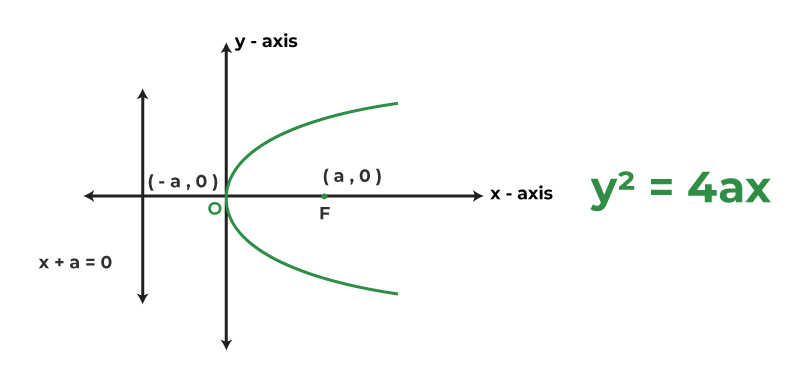
\includegraphics[width=0.6\textwidth]{parabola.png}
\begin{itemize}
    \item Symmetrix about the $x$-axis
    \item Focus at $(a, 0)$
    \item Vertex at $(0, 0)$
\end{itemize}
\subsection{Definition}
\begin{itemize}
    \item The locus of points that are the \textbf{same distance} from a fixed point, $S$,
          called the \textbf{focus}, and a fixed straight line called the \textbf{directrix}
    \item $\dfrac{\text{distance to foci}}{\text{distance to directrix}} = e = 1$
\end{itemize}
\subsection{Cartesian equation}
\begin{itemize}
    \item $y^2=4ax$ ($a>0$)
\end{itemize}
\subsection{Parametric equation}
\begin{itemize}
    \item $x=at^2$
    \item $y=2at$
    \item $t\in \Rset$
\end{itemize}
\subsection{Eccentricity}
\begin{itemize}
    \item $e=1$
\end{itemize}
\subsection{Directrix}
\begin{itemize}
    \item The directrix has equation $x+a=0$
\end{itemize}
\subsection{Tangents and normals}
\begin{itemize}
    \item $\dfrac{\dy}{\dx} = \frac{1}{t} = \frac{2a}{y}$
    \item Equation of tangent: $ty=x+at^2$ at $P(at^2, 2at)$
    \item Equation of normal: $y+tx=2at+at^3$ at $P(at^2, 2at)$
\end{itemize}

\section{Rectangular hyperbolas}
\subsection{Graph}
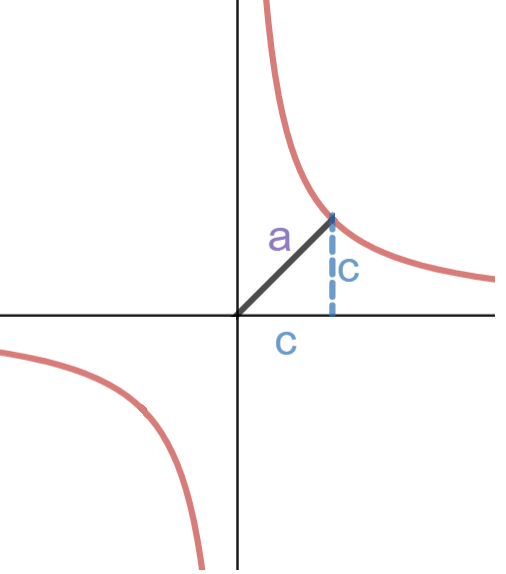
\includegraphics[width=0.3\textwidth]{rectangular_hyperbola.png}
\begin{itemize}
    \item Asymptotes at $x=0$ and $y=0$ ($x$ and $y$-axis)
\end{itemize}
\subsection{Definition}
\begin{itemize}
    \item The locus of points that are the \textbf{same distance} from a fixed point, $S$,
          called the \textbf{focus}, and a fixed straight line called the \textbf{directrix}
    \item $\dfrac{\text{distance to foci}}{\text{distance to directrix}} = e = 1$
\end{itemize}
\subsection{Cartesian equation}
\begin{itemize}
    \item $xy=c^2$ ($c>0$)
\end{itemize}
\subsection{Parametric equation}
\begin{itemize}
    \item $x=ct$
    \item $y=\frac{c}{t}$
    \item $t \neq 0, t\in\Rset$
\end{itemize}
\subsection{Eccentricity}
\begin{itemize}
    \item $e=\sqrt{2}$
\end{itemize}
\subsection{Directrix}
\begin{itemize}
    \item $x+y=\pm c\sqrt{2}$
\end{itemize}
\subsection{Tangents and normals}
\begin{itemize}
    \item Equation of tangent: $x+t^2y=2ct$ at $P\left(ct, \frac{c}{t}\right)$ or
    $y\times y_0 = 4p \left(\frac{x+x_0}{2}\right)$ at $(y_0, x_0)$
    \item Equation of normal: $t^3x-ty=c\left(t^4-1\right)$ at $P\left(ct, \frac{c}{t}\right)$
\end{itemize}

\section{Reciprocal equations}
\subsection{$y=\frac{k}{x}$}
\begin{itemize}
    \item $x=t$
    \item $y=\dfrac{k}{t}$
    \item Asymptotes: $y=0$, $x=0$
\end{itemize}

\subsection{$y=ax+\frac{b}{x}$}
\begin{itemize}
    \item Asymptotes: $y=ax$, $x=0$
\end{itemize}
\chapter{Conic sections 2}
\section{Ellipse}
\subsection{Graph}
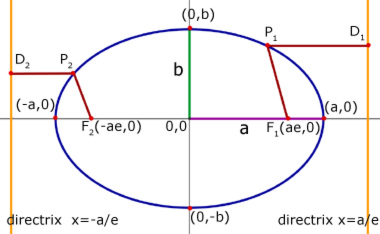
\includegraphics[width=0.4\textwidth]{ellipse.png}
\subsection{Definition}
\begin{itemize}
    \item $PF_1 + PF_2 = 2a$
    \item $\dfrac{\text{distance from point $P$ to a focus}}{\text{distance from the same point to the corresponding directrix}}=e=\frac{c}{a}$
\end{itemize}
\subsection{Cartesian equation}
\begin{description}
    \item[Centre $(0,0)$] $\dfrac{x^2}{a^2}+\dfrac{y^2}{b^2}=1$
    \item[Centre $(h,k)$] $\dfrac{(x-h)^2}{a^2}+\dfrac{(y-k)^2}{b^2}=1$
\end{description}
\subsection{Parametric equation}
\begin{description}
    \item[Centre $(0,0)$] $x=a\cos t$, $y=b\sin t$ ($0\leq t < 2\pi$)
    \item[Centre $(h,k)$] $x=h+a\cos t$, $y=k+b\sin t$ ($0\leq t < 2\pi$)
\end{description}
\subsection{Eccentricity}
\begin{itemize}
    \item $e=\frac{c}{a}=\sqrt{1-\frac{b^2}{a^2}}$
    \item $0<e<1$
\end{itemize}
\subsection{Directrix}
\begin{itemize}
    \item $x=h\pm \dfrac{a^2}{c} = h\pm\frac{a}{e}$
    \item $(h-c, 0)$ corresponds to $x=h-\frac{a}{e}$, $(h+c, 0)$ corresponds to $x=h+\frac{a}{e}$
\end{itemize}
\subsection{Tangents and normals}
\begin{itemize}
    \item Equation of tangent: $bx\cos t + ay\sin t = ab$ at $P(a\cos t, b\sin t)$
    \item Equation of normal: $ax\sin t - by\cos t=(a^2-b^2)\cos t\sin t$ at $P(a\cos t, b\sin t)$
\end{itemize}
\subsection{Chord length}
For chord $AB$ with gradient $m$:
\begin{align*}
    |AB|&=\sqrt{(1+m^2)(x_1-x_2)^2}\\
    &=\sqrt{1+m^2}\times\sqrt{(x_1+x_2)^2-4x_1x_2}
\end{align*}
\subsection{Circumference}
\begin{align*}
    C &= 4\int_{0}^{\frac{\pi}{2}}\sqrt{\left(\frac{\dx}{\dtheta}\right)^{2}+\left(\frac{\dy}{\dtheta}\right)^{2}}\dtheta\\
    &= 4a\int_{0}^{\frac{\pi}{2}}\sqrt{1-e^2\cos^2\theta}\dtheta\\
    &\approx \pi\left[3(a+b)-\sqrt{(3a+b)(3b+a)}\right]
\end{align*}

\section{Hyperbola}
\subsection{Graph}
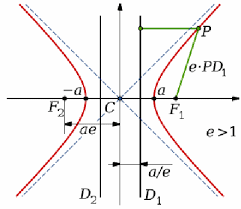
\includegraphics[width=0.4\textwidth]{hyperbola.png}
\begin{itemize}
    \item Asymptotes at $y=\pm \frac{b}{a}x$
\end{itemize}
\subsection{Definition}
\begin{itemize}
    \item $|PF_1 - PF_2| = 2a$
\end{itemize}
\subsection{Cartesian equation}
\begin{description}
    \item[Centre $(0,0)$] $\dfrac{x^2}{a^2}-\dfrac{y^2}{b^2}=1$ ($b^2=c^2-a^2$)
    \item[Centre $(h,k)$] $\dfrac{(x-h)^2}{a^2}-\dfrac{(y-k)^2}{b^2}=1$
\end{description}
\subsection{Parametric equation}
\subsubsection{Using $\sec$ and $\tan$}
\begin{description}
    \item[Centre $(0,0)$] $x=a\sec t$, $y=b\tan t$
    \item[Centre $(h,k)$] $x=h+a\sec t$, $y=k+b\tan t$
    \item[Domain] $t\neq \frac{\pi}{2}+k\pi$
\end{description}
\subsubsection{Using $\cosh$ and $\sinh$}

\begin{description}
    \item[Centre $(0,0)$] $x=\pm a\cosh t$, $y=b\sinh t$
    \item[Centre $(h,k)$] $x=h\pm a\cosh t$, $y=k+b\sinh t$
    \item[Domain] $t \in \mathbb{R}$
\end{description}
\subsection{Eccentricity}
\begin{itemize}
    \item $e=\frac{c}{a}=\sqrt{1-\frac{b^2}{a^2}}$
    \item $e>1$
\end{itemize}
\subsection{Directrix}
\begin{itemize}
    \item $x=h\pm \dfrac{a^2}{c} = h\pm\frac{a}{e}$
    \item $(h-c, 0)$ corresponds to $x=h+\frac{a}{e}$, $(h+c, 0)$ corresponds to $x=h-\frac{a}{e}$
\end{itemize}
\subsection{Tangents and normals}
\subsubsection{Tangent equations}
\begin{itemize}
    \item $ay\sinh t + ab = bx\cosh t$ at $P(a\cosh t, b\sinh t)$
    \item $bx\sec\theta-ay\tan\theta = ab$ at $P(a\sec\theta, b\tan\theta)$
\end{itemize}
\subsubsection{Normal equations}
\begin{itemize}
    \item $ax\sinh t + by\cosh t = (a^2+b^2)\sinh t\cosh t$ at $P(a\cosh t, b\sinh t)$
    \item $by + ax\sin\theta = (a^2+b^2)\tan\theta$ at $P(a\sec\theta, b\tan\theta)$
\end{itemize}

\section{Finding the type of the quadratic curve}
For curve $ax^2+bxy+cy^2+dx+ey+f=0$:
\begin{itemize}
    \item Find the determinant: $\Delta = b^2-4ac$
    \item $\Delta < 0$: ellipse if $a\neq c$ or $b\neq 0$, circle if $a=c$ and $b=0$
    \item $\Delta = 0$: if $a=c=0$ then a straight line, otherwise parabola
    \item $\Delta > 0$: $a=-c$ and $b=0$: intersecting lines, otherwise hyperbola
\end{itemize}
\chapter{Inequalities}
\section{Triangle inequalities}
$$\left| a \right|-\left| b \right| \leq \left| a\pm b \right| \leq \left| a \right| + \left| b \right|$$


\section{Modulus inequalities}
\subsection{Common methods}
\begin{itemize}
    \item $\left|f(x)\right|\geq g(x)$: $f(x) \geq g(x)$ or $f(x) \leq -g(x)$
    \item $\left|f(x)\right|\leq g(x)$: $-g(x) \leq f(x) \leq g(x)$ or square both sides
          (solution only exists when $g(x) \geq 0$ so no solution is omitted)
    \item $\left|f(x)\right|\leq \left|g(x)\right|$: $f(x)^2 < \leq g(x)^2$
    \item $\left|f(x)\right| + \left|g(x)\right| \leq m(x)$: solve each interval separately
\end{itemize}

\subsection{Things to consider}
\begin{enumerate}
    \item Sketching graphs
    \item Finding critical values
    \item Rearranging the inequality
\end{enumerate}
\chapter{The $t$-formulae}
\section{$t$-substitution formulae}
When $t=\tan\left(\frac{\theta}{2}\right)$:
\begin{itemize}
    \item $\sin\theta = \frac{2t}{1+t^2}$
    \item $\cos\theta = \frac{1-t^2}{1+t^2}$
    \item $\tan\theta = \frac{2t}{1-t^2}$
\end{itemize}

\section{Uses}
\begin{itemize}
    \item Trigometric equations
    \item Integration / differentiation
\end{itemize}

\chapter{Taylor series}
\section{Taylor series}
$$f(x+a) = f(a)+f'(a)x + \frac{f''(a)x^2}{2!}+\dots+\frac{^{(r)}(a)x^r}{r!}+\dots$$
$$f(x)=f(a)+f'(a)(x-a)+\frac{f''(a)(x-a)^2}{2!}+\dots+\frac{f^{(r)}(a)(x-a)^r}{r!}+\dots$$

\section{Finding limits}
Given $\lim_{x\rightarrow a} f(x)=L$ and $\lim_{x\rightarrow a} g(x)=M$:
\begin{itemize}
    \item $\lim_{x\rightarrow a} cf(x)=cL$ ($c$ is a constant)
    \item $\lim_{x\rightarrow a} \left(f(x)+g(x)\right)=L+M$
    \item $\lim_{x\rightarrow a} f(x)g(x)=LM$
    \item $\lim_{x\rightarrow a} \frac{f(x)}{g(x)}=\frac{L}{M}$
\end{itemize}

\section{Series solution of differential equations}

\chapter{Methods in calculus}
\section{Linear transformations in 2D}
\subsection{Properties}
If $L(\vec{v})$ is linear:
\begin{enumerate}
	\item $L(\vec{v})$ should always map the origin onto itself
	\item $L(\vec{v})$ can be represented by a matrix
	\item $L(\vec{v_1}+\vec{v_2})=L(\vec{v_1})+L(\vec{v_2})$ (closure in addition)
	\item $L(\lambda\vec{v_1})=\lambda L(\vec{v_1})$ (closure in scalar multiplication)
\end{enumerate}
\subsection{Invariant points and lines}
\begin{description}
	\item[Invariant points:] Points which are mapped onto themselves under the given transformation
	\item[Invariant lines:] Lines which map onto themselves
\end{description}

\subsection{Reflection}
\begin{description}
	\item[Reflection in $y$-axis:] $\begin{pmatrix}
		-1&0\\0&1
	\end{pmatrix}$, invariant points: points on the $y$-axis; invariant lines: $x=0$, $y=k$
	\item[Reflection in $x$-axis:] $\begin{pmatrix}
		1&0\\0&-1
	\end{pmatrix}$, invariant points: points on the $x$-axis; invariant lines: $y=0$, $x=k$
	\item[Reflection in line $y=x$:] $\begin{pmatrix}
		0&1\\1&0
	\end{pmatrix}$, invariant points: points on $y=x$; invariant lines: $y=x$, $y=-x+k$
	\item[Reflection in line $y=-x$:] $\begin{pmatrix}
		0&-1\\-1&0
	\end{pmatrix}$, invariant points: points on $y=-x$; invariant lines: $y=-x$, $y=x+k$
\end{description}

\subsection{Rotation}
\begin{description}
	\item[Rotation through angle $\theta$ anticlockwise about the origin] $\begin{pmatrix}
		\cos\theta&-\sin\theta\\\sin\theta&\cos\theta
	\end{pmatrix}$
	\item[Invariant points:] Only $(0,0)$
	\item[Invariant lines:] When $\theta=180\textdegree$ any line passing through the origin is an invariant line, otherwise no invariant lines
\end{description}

\subsection{Enlargement / stretches}
\begin{description}
	\item[Transformation matrix] $\begin{pmatrix}
		a & 0 \\ 0 & b
	\end{pmatrix}$ = a stretch of scale factor $a$ parallel to the $x$-axis and scale factor $b$ parallel to the $y$-axis
	\item[Invariant lines] $x$- and $y$-axes for all stretches
	\begin{itemize}
		\item Stretch parallel to the $x$-axes: any line parallel to the $x$-axes
		\item Stretch parallel to the $y$-axes: any line parallel to the $y$-axes
	\end{itemize}
	\item[Invariant points] The origin is always an invariant point
	\begin{itemize}
		\item Stretch parallel to the $x$-axes: points on the $y$-axes
		\item Stretch parallel to the $y$-axes: points on the $x$-axes
	\end{itemize}
	\item[Change in area] $\det(\mathbf{M}) = \text{area scale factor}$
\end{description}

\section{Linear transformations in 3D}
\begin{description}
	\item[Reflection in plane $x=0$] $\begin{pmatrix}
		-1 & 0 & 0\\
		0 & 1 & 0 \\
		0 & 0 & 1
	\end{pmatrix}$
	\item[Reflection in plane $y=0$] $\begin{pmatrix}
		1 & 0 & 0\\
		0 & -1 & 0 \\
		0 & 0 & 1
	\end{pmatrix}$
	\item[Reflection in plane $z=0$] $\begin{pmatrix}
		1 & 0 & 0\\
		0 & 1 & 0 \\
		0 & 0 & -1
	\end{pmatrix}$
	\item[Rotation angle $\theta$ anticlockwise about the $x$-axis] $\begin{pmatrix}
		1 & 0 & 0\\
		0 & \cos\theta & -\sin\theta \\
		0 & \sin\theta & \cos\theta
	\end{pmatrix}$
	\item[Rotation angle $\theta$ anticlockwise about the $y$-axis] $\begin{pmatrix}
	\cos\theta & 0 & \sin\theta \\
	0 & 1 & 0\\
	-\sin\theta & 0 & \cos\theta
	\end{pmatrix}$
	\item[Rotation angle $\theta$ anticlockwise about the $z$-axis] $\begin{pmatrix}
		\cos\theta & -\sin\theta & 0\\
		\sin\theta & \cos\theta & 0\\
		0 & 0 & 1
	\end{pmatrix}$
\end{description}





\chapter{Numerical methods}
\section{Hyperbolic function definitions}
\subsection{$\sinh x$}
\begin{description}
	\item[Definition] $\sinh x = \dfrac{e^x-e^{-x}}{2}$
	\item[Domain] $x \in \textbf{R}$
	\item[Asymptotes] $x\rightarrow +\infty$, $y\rightarrow\dfrac{e^x}{2}$; $x\rightarrow -\infty$, $y\rightarrow -\dfrac{e^{-x}}{2}$
	\item[x-intercept] $(0,0)$
	\item[y-intercept] $(0,0)$
	\item[Graph]
\end{description}

\subsection{$\cosh x$}
\begin{description}
	\item[Definition] $\cosh x = \dfrac{e^x+e^{-x}}{2}$
	\item[Domain] $x \in \textbf{R}$
	\item[Asymptotes] $x\rightarrow +\infty$, $y\rightarrow\dfrac{e^x}{2}$; $x\rightarrow -\infty$, $y\rightarrow\dfrac{e^{-x}}{2}$
	\item[x-intercept] No
	\item[y-intercept] $(0,1)$
	\item[Graph]
\end{description}

\subsection{$\tanh x$}
\begin{description}
	\item[Definition] $\tanh x = \dfrac{\sinh x}{\cosh x}=\dfrac{e^x-e^{-x}}{e^x+e^{-x}}$
	\item[Domain] $x \in \textbf{R}$
	\item[Asymptotes] $x\rightarrow +\infty$, $y\rightarrow 1$; $x\rightarrow -\infty$, $y\rightarrow -1$
	\item[x-intercept] $(0,0)$
	\item[y-intercept] $(0,0)$
	\item[Graph]
\end{description}

\subsection{$\csch x$}
\begin{description}
	\item[Definition] $\csch x = \dfrac{1}{\sinh x}$
	\item[Domain] 
	\item[Asymptotes] 
	\item[x-intercept] 
	\item[y-intercept] 
	\item[Graph]
\end{description}


\subsection{$\sech x$}
\begin{description}
	\item[Definition] $\sech x = \dfrac{1}{\cosh x}$
	\item[Domain] 
	\item[Asymptotes] 
	\item[x-intercept] 
	\item[y-intercept] 
	\item[Graph]
\end{description}


\subsection{$\coth x$}
\begin{description}
	\item[Definition] $\coth x = \dfrac{\cosh x}{\sinh x}$
	\item[Domain] 
	\item[Asymptotes] 
	\item[x-intercept] 
	\item[y-intercept] 
	\item[Graph]
\end{description}

\section{Identities of hyperbolic functions}
Similar to trigonometric identities:
\begin{itemize}
	\item $\tanh x = \dfrac{\sinh x}{\cosh x}$
	\item $\cosh^2 x - \sinh^2 x = 1$
	\item $\tanh^2 x + \sech^2 x= 1$
	\item $\coth^2 x - \csch^2 x = 1$
\end{itemize}

\subsection{Addition}
\begin{itemize}
	\item $\sinh(x+y)=\sinh x \cosh y + \sinh y \cosh x$
	\item $\cosh(x+y)=\cosh x \cosh y + \sinh x \sinh y$
	\item $\tanh(x+y) = \dfrac{\sinh(x+y)}{\cosh(x+y)} = \dfrac{\sinh x \cosh y + \sinh y \cosh x}{\cosh x \cosh y + \sinh x \sinh y} = \dfrac{\frac{\sinh x}{\cosh x}+\frac{\sinh y}{\cosh y}}{1 + \frac{\sinh x \sinh y}{\cosh x \cosh y}}=\dfrac{\tanh x + \tanh y}{1 + \tanh x \tanh y}$
\end{itemize}

\subsection{Double angle}
\begin{itemize}
	\item $\sinh 2x = 2\sinh x \cosh x$
	\item $\cosh 2x = \cosh^2 x + \sinh^2 x = 2\cosh^2 x - 1 = 2\sinh^2 + 1$
	\item $\tanh 2x = \dfrac{2\tanh x}{1 + \tanh^2 x}$
\end{itemize}

\subsection{Power descending}


\section{Differentiating hyperbolic functions}
\begin{itemize}
	\item $(\sinh x)'=\cosh x$
	\item $(\cosh x)'=\sinh x$
	\item $(\tanh x)'=1-\tanh^2 x = \sech^2 x$
	\item $(\csch x)'=-\coth x \csch x$
	\item $(\sech x)'=-\sech x \tanh x$
	\item $(\coth x)'=-\sech^2 x$
\end{itemize}
\chapter{Redicible differential equations}
\section{SUVAT equations}
\begin{itemize}
    \item $s=ut+\dfrac{1}{2}at^2$
    \item $s=vt-\dfrac{1}{2}at^2$
    \item $v=u+at$
    \item $v^2=u^2+2as$
    \item $s=\dfrac{1}{2}(u+v)t$
\end{itemize}



\end{document}